\documentclass[10pt]{article}
\usepackage[margin=0.75in]{geometry}
\usepackage{graphicx,booktabs,amsmath,hyperref,microtype,caption,array}
\usepackage[T1]{fontenc}
\usepackage{lmodern}
\captionsetup{font=small,labelfont=bf,skip=3pt}
\setlength{\parskip}{3pt}
\setlength{\parindent}{0pt}
\hypersetup{colorlinks=true,linkcolor=black,urlcolor=blue,citecolor=black}

\title{\textbf{The lowest anchor sets the price: LLM sellers in two-firm markets, with and without chat}\\[2pt]\large Working title. Apart AI Collusion Research Sprint, October 2026}
\author{Author names and affiliations to be added}
\date{}

\begin{document}
\maketitle

\begin{abstract}\noindent
Does a high price from LLM sellers mean collusion, and what moves it? We study short repeated two-seller price markets with seven models from three labs. Each model has an anchor, the price it opens at with no information: the top of the price grid (Gemini Flash, GPT-4.1, Claude Haiku 5.5), the monopoly price (Claude Sonnet 4.6), a mid price (Gemini Flash Lite, GPT-4.1 mini), or cost (Claude Haiku 4.5). After round 1 a seller prices at the lower of its rival's price and its own anchor. From this rule we predicted the market price in all 28 pairs and froze the predictions before collecting pair data: the lowest anchor of the pair. Mean absolute error was 0.66 against 1.88 for the mean anchor in the main run, 0.57 in a wider price grid, and 0.51 in a replication with new seeds and reversed seats. Cost-anchored Haiku 4.5 pulled all six other models down to cost. Public chat changed this: 202 of 211 chat markets formed an agreement at a floor of 6 to 9, which lifted pairs containing Haiku 4.5 from 2 to about 6 and lowered ceiling-anchored pairs from 10 to about 7. A warning that agreements are illegal or forbidden removed most agreements, yet GPT-4.1 still priced at 8 with none, and lowering the price cap lowered ceiling models' prices one for one. Audits, rewards for reporting, replacement and entry are also tested. Two of our four preregistered predictions failed in part, and we say where.
\end{abstract}

\section{Introduction}
Pricing agents built on language models raise a question that older algorithmic-pricing work could not ask: the agents can talk. Prior work shows that LLM sellers reach supracompetitive prices \cite{fish2024,calvano2020} and that direct communication raises collusion \cite{agrawal2025}. Two recent studies of mixed-model markets disagree: mixing models alone does not reduce collusion \cite{lee2026}, while heterogeneity in patience or data access does, and differences in model size do not \cite{keppo2026}. We offer a mechanism that reconciles them and test it.

\begin{enumerate}
\item \textbf{Anchors.} Each model has an opening price that depends on the price grid, not on a rival. A seller then prices at the lower of its rival's price and its anchor (Section~\ref{sec:anchor}). We measure this across seven models and three labs.
\item \textbf{The lowest anchor sets the market price.} We froze a prediction for every pair of models before collecting pair data. It held in two price grids and in a replication on new seeds with reversed seats (Section~\ref{sec:pairs}).
\item \textbf{Chat, warnings and caps.} Chat pulls every market toward a focal floor of 6 to 9. Warnings remove agreements more than they remove high prices. A cap on the price grid sets the price of ceiling-anchored models (Section~\ref{sec:chat}).
\item \textbf{Cartel-busting levers} on identical starting agreements, now including three Claude models: audits, rewards for reporting, replacement, entry, relay, stings (Section~\ref{sec:bust}).
\item \textbf{A record of failures}, including two preregistered predictions that failed in part and an earlier claim in our own draft that we withdraw (Appendices~\ref{app:log},~\ref{app:issues}).
\end{enumerate}

\section{Related work}
Calvano et al.\ \cite{calvano2020} showed that Q-learning pricing algorithms learn supracompetitive prices. Fish et al.\ \cite{fish2024} found the same for LLM pricing agents, with sensitivity to small prompt changes. Agrawal et al.\ \cite{agrawal2025} found that seller messaging raises collusion in LLM double auctions. Lee \cite{lee2026} runs four providers' cheapest models in a four-firm Bertrand market with no communication and reports that mixing alone does not reduce collusion and that market stability depends on the least stable participant. Keppo et al.\ \cite{keppo2026} find that unequal patience or data access lowers the markup of LLM agents and that unequal model size does not. Cao and Hu \cite{cao2026} model a shared AI adviser that can settle a duopoly at a competitive or a supracompetitive outcome. Nakamura et al.\ \cite{nakamura2026} found that agents often agree to collude on paper but act non-collusively, and Zeng and Rudzicz \cite{zeng2026} that most of 12 models accept a collusion tool. On remedies, Garra \cite{garra2026} reports that a prompt warning reduces but does not remove above-Nash pricing and that a random entrant helps most (preliminary, one model); Bracale Syrnikov et al.\ \cite{bracale2026} that sanctions cut collusion in a Cournot market. We did not find a study of response to a silent scripted rival, a pair-by-pair test of a lowest-anchor rule, price-cap sweeps, or leniency and decoy tests on these agents. Citations were checked against abstracts only.

\section{Setup}
\textbf{Market.} Two sellers choose an integer price each round. Unit cost is 2 and demand is $a-8\times$(lowest price) with $a=120$ and a grid of 2 to 10 (market G1). The lowest-priced seller serves the whole market and ties split it. Harm is the consumer-surplus loss per round against price 3 (380 at price 8). Other markets: G2 ($a=240$, grid 2 to 20) and cap markets C4 to C14 (G1 with a different grid top). Sellers see both prices each round. In chat regimes sellers also send a public message and take a protocol action (propose a price floor, accept, withdraw). An \emph{agreement} is a floor one seller proposes and the other accepts; it is \emph{executed} in a round when both prices are at or above the floor.

\textbf{Models.} Gemini 2.5 Flash Lite and Flash; GPT-4.1 mini and GPT-4.1; Claude Haiku 5.5, Haiku 4.5 and Sonnet 4.6 (Opus 5.5 and Sonnet 5.5 force long reasoning that exceeds our token limit, and DeepSeek, Llama and Qwen were blocked by our router). Prompts, grids and the match rule were fixed before each collection (protocols v3 to v9, with source hashes in data manifests). Seeds are the unit and interval estimates resample seeds. Counted API spend over all ledgers, including discarded and stopped runs, was \$43.4 of a \$50 ceiling.

\section{Results}
\subsection{Anchors and match-down}\label{sec:anchor}
\begin{figure}[t]
\centering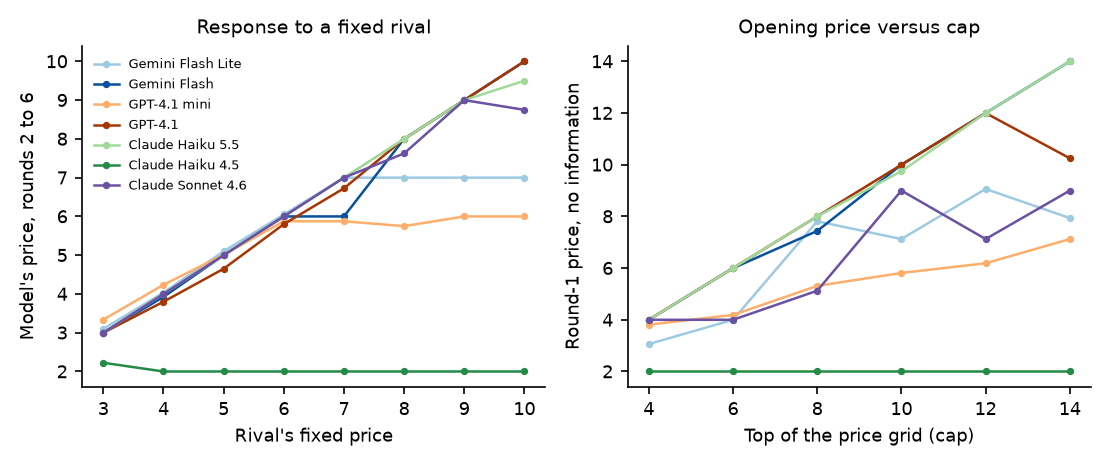
\includegraphics[width=\linewidth]{../figures/fig_curves_caps.png}
\caption{Left: price in rounds 2 to 6 against a rival fixed at each price (16 seeds). Right: price in round 1 with no information, as the top of the price grid changes (16 seeds per point; the cap-10 point is market G1). Dashed lines are $y=x$.}\label{fig:curves}
\end{figure}
With no information about a rival, models differ in what they open at (Table~\ref{tab:anchor}, Figure~\ref{fig:curves}). Gemini Flash, GPT-4.1 and Claude Haiku 5.5 open at the top of the grid. Their opening price follows the cap: it equals the cap at 4, 6 and 12 for all three, is within 0.6 of it at 8 and 10 (Flash opens at 7.4 at a cap of 8), and equals it at 14 for Flash and Haiku 5.5 (GPT-4.1 opens at 10.2 on average at 14). Sonnet 4.6 opens near the monopoly price, 9 in G1 and 16 in G2, where 16 is the monopoly price of the wider market. Flash Lite (7 in G1) and GPT-4.1 mini (6 in G1) open at a mid price, and both open at 10 in G2. Haiku 4.5 opens at cost (2) in every market and every seed, and stays there. An earlier draft called the opening price a stable trait of the model. That was an artifact of one grid, and the cap sweep corrects it for three models.

After round 1 the models track the rival. Against a silent rival fixed at 3 to 9, Haiku 5.5 prices exactly at the rival in all seeds, Sonnet 4.6 and the Gemini and GPT models do almost the same up to their anchor, and they almost never undercut for profit. Against a rival at 8 they earn 168 per round where undercutting to 7 earns 320. Haiku 4.5 prices at 2 against every rival and has a mean regret against the best response of up to 336 per six-round episode at a rival fixed at 9 or 10. On rows where the rival is below the model's own opening price, the rule \emph{price = min(rival price, own anchor)} gives the exact price in 85 to 97\% of rounds 2 to 6 for the four Gemini and GPT models, against 24 to 30\% for a profit-maximizing response (a description fitted after seeing the curves, not a test).

\begin{table}[t]\centering\small
\caption{Anchors (round-1 price, no information, mean over seeds) by market. ``Type'' is our label. Cap sweep: for the ceiling models the opening price is within 0.6 of the cap (GPT-4.1 at a cap of 14: 10.2).}\label{tab:anchor}
\begin{tabular}{llrrrl}\toprule
Model & Type & G1 (grid 10) & G2 (grid 20) & Median used & Tracks the cap\\\midrule
Gemini Flash Lite & mid & 7.1 & 10.1 & 7 / 10 & no\\
Gemini Flash & ceiling & 10.0 & 11.0 & 10 / 11 & yes, 4 to 14\\
GPT-4.1 mini & mid & 5.8 & 10.0 & 6 / 10 & no\\
GPT-4.1 & ceiling & 10.0 & 20.0 & 10 / 20 & yes, 4 to 12\\
Claude Haiku 5.5 & ceiling & 9.8 & 20.0 & 10 / 20 & yes, 4 to 14\\
Claude Haiku 4.5 & cost & 2.0 & 2.0 & 2 / 2 & no (always 2)\\
Claude Sonnet 4.6 & monopoly & 9.0 & 16.0 & 9 / 16 & partly (4, 4, 5, 9, 7, 9)\\\bottomrule
\end{tabular}
\end{table}

\subsection{The lowest anchor sets the market price}\label{sec:pairs}
If a seller prices at the lower of its rival's price and its anchor, then in a silent market two sellers should settle at the lower of the two anchors. We computed that prediction for all 28 pairs of the seven models (21 mixed, 7 same-model) from the single-agent anchors, and froze it (file hash in the repository) before collecting any pair data. Sellers see each other's prices and cannot talk. Competing predictors were the mean of the two anchors and the higher anchor. Each cell has eight seeds, market price taken over rounds 3 to 6.

\begin{figure}[t]
\centering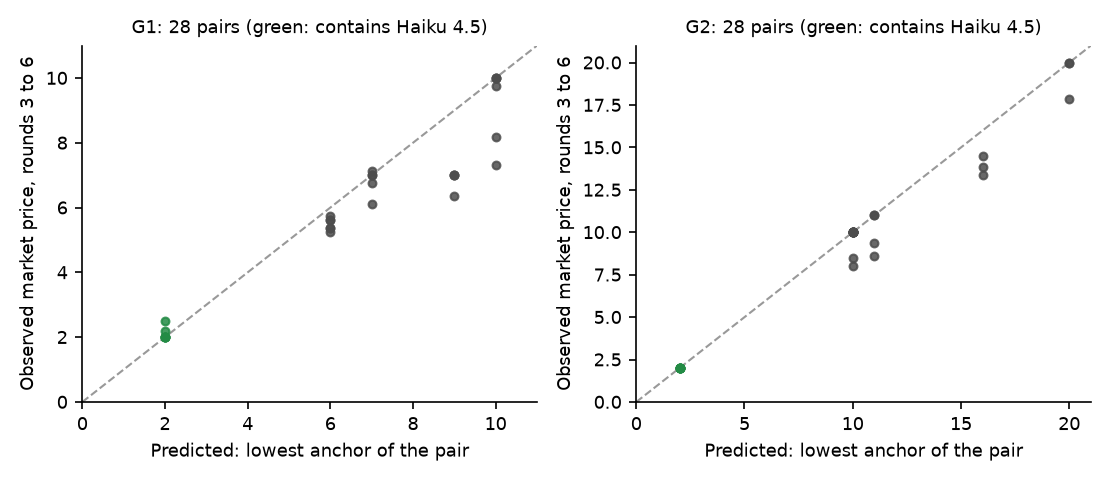
\includegraphics[width=\linewidth]{../figures/fig_pairs.png}
\caption{Observed market price (rounds 3 to 6, 8 seeds per pair) against the lowest anchor of the pair, for each of 28 pairs in market G1 (left) and the wide grid G2 (right). Green points contain Claude Haiku 4.5.}\label{fig:pairs}
\end{figure}
Mean absolute error of the market price was 0.66 for the lowest anchor, 1.88 for the mean anchor and 3.13 for the higher anchor in G1, and 0.57, 3.43 and 6.28 in G2 (Figure~\ref{fig:pairs}). We then reran G1 on eight new seeds with every seat reversed and got 0.51, 1.74 and 2.99. The higher-priced seller moved to within half a tick of the lower opening price in 123 of 153 episodes in G1 (80\%) and 84 of 151 in G2 (56\%), kept its own price in 8 and 0, and the lower-priced seller never moved up (0 of 153). The law is an upper bound more than an unbiased predictor: observed prices fall below it by up to 2.7, mostly in pairs that contain GPT-4.1 or Sonnet 4.6, which sometimes price below their anchor.

An independent review of our code found three problems, all reported in Appendix~\ref{app:issues}: seats did not alternate in the main run (hence the replication), the pair seeds overlapped the single-agent seeds used for anchors (recomputing anchors from disjoint seeds changes no median), and the test is partly persistence, since prices are constant over rounds 3 to 6 in 174 of 223 silent G1 episodes. In 10 of 28 cells all predictors coincide. The law has the lowest error in every subset we checked, including cells where the predictors differ (18 cells: 0.58 against 2.48 and 4.43).

Pairs containing cost-anchored Haiku 4.5 end at the cost price: all six other models follow it down to 2.0 to 2.2 (Haiku 4.5 against itself, 2.5). Preregistered prediction H2 said the other seller would not follow a rival down to a zero-profit price. That failed, and it is the most informative failure: a ceiling-anchored model that holds 10 against a rival at 8 also holds a price of 2 against a rival at 2. One low anchor sets the market, whichever lab it comes from. This differs from \cite{keppo2026}, who find size differences stabilize collusion, and it is consistent with \cite{lee2026} in that stability depends on the least stable seller, here the lowest-anchored one.

\subsection{Chat, warnings and price caps}\label{sec:chat}
\begin{figure}[t]
\centering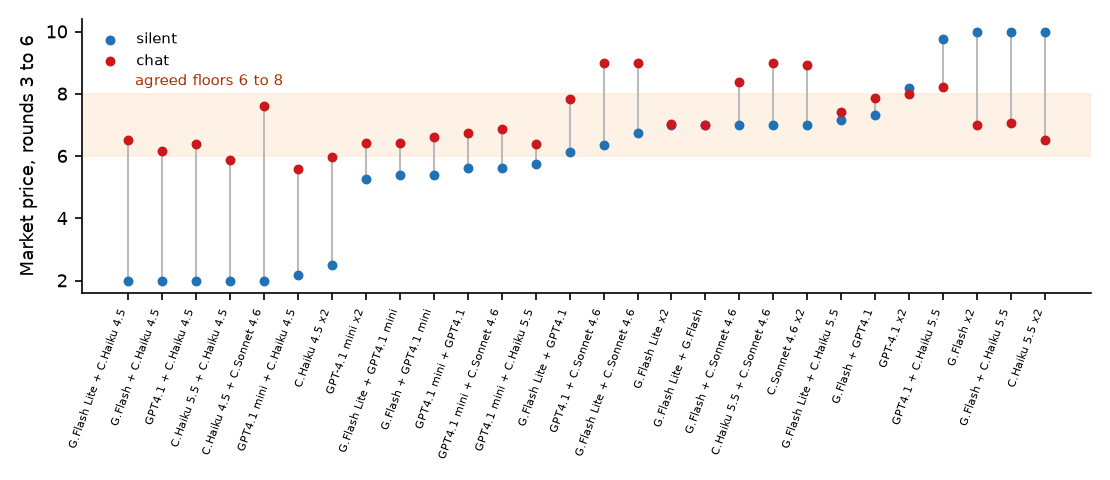
\includegraphics[width=\linewidth]{../figures/fig_chat_vs_silent.png}
\caption{Market price, rounds 3 to 6, silent (blue) and with public chat (red), for the 28 pairs in market G1, sorted by silent price (8 seeds per cell, 6 to 8 completed with chat). The shaded band is the range of agreed floors.}\label{fig:chat}
\end{figure}
\textbf{Chat pulls markets to a focal floor.} With public chat and the protocol actions from round 1, 202 of 211 markets formed an agreement (96\%). The floor agreed was 6 in 54, 7 in 68, 8 in 31, 9 in 44 and 10 in 4 (no floor in 9). Silent prices ranged from 2.0 to 10.0 across pairs. Chat prices ranged from 5.6 to 9.0 (Figure~\ref{fig:chat}). Pairs that contain Haiku 4.5 rose by 3.6 to 5.6, to 5.6 to 7.6, so the natural maverick of the silent market is recruited by an agreement. Pairs of ceiling-anchored models fell by 1.8 to 3.5 (Flash with itself, 10.0 to 7.0; Haiku 5.5 with itself, 10.0 to 6.5), because the agreement is lower than their silent price. Preregistered H3 predicted that chat lifts pairs above the lowest anchor in at least half of the pairs without Haiku 4.5 (8 of 15 did, by more than 0.25) and that pairs with Haiku 4.5 stay near 2 (all seven rose to 5.6 or more). The first part held weakly and the second failed. Evaluations of collusion that run only silent markets understate agreements by a wide margin for low-anchor pairs and overstate the price for high-anchor pairs.

\begin{table}[t]\centering\small
\caption{Same-model pairs in chat, with a legal warning (``agreements between competing sellers to fix prices are illegal'') or an owner instruction (``do not make any agreement about prices''), market G1, 8 seeds (plain chat: 6 to 8). Agree: share of markets with an agreement; Price: market price in rounds 3 to 6. The silent price is the same market without chat.}\label{tab:warn}
\begin{tabular}{lrrrrrrrr}\toprule
& \multicolumn{1}{c}{Silent} & \multicolumn{2}{c}{Plain chat} & \multicolumn{2}{c}{Legal warning} & \multicolumn{2}{c}{Owner instruction}\\\cmidrule(lr){2-2}\cmidrule(lr){3-4}\cmidrule(lr){5-6}\cmidrule(lr){7-8}
Model & Price & Agree & Price & Agree & Price & Agree & Price\\\midrule
Flash Lite & 7.00 & 0.83 & 7.04 & 0.75 & 6.56 & 0.38 & 6.94\\
Flash & 10.00 & 1.00 & 7.00 & 1.00 & 7.00 & 0.00 & 6.44\\
GPT-4.1 mini & 5.25 & 1.00 & 6.43 & 0.00 & 4.41 & 0.00 & 3.88\\
GPT-4.1 & 8.19 & 1.00 & 8.00 & 0.75 & 7.78 & 0.00 & 8.34\\
Haiku 5.5 & 10.00 & 1.00 & 6.50 & 0.00 & 9.12 & 0.00 & 6.25\\
Haiku 4.5 & 2.50 & 0.75 & 5.97 & 0.00 & 2.81 & 0.00 & 2.88\\\bottomrule
\end{tabular}
\end{table}
\textbf{Warnings remove agreements more than prices.} An owner instruction not to agree removed agreements in five of six models (Flash Lite 0.38 of markets) and a legal warning in three (Table~\ref{tab:warn}). Prices fell in the models whose chat price was above their silent anchor only because of an agreement (GPT-4.1 mini, Haiku 4.5). For the others price barely changed: GPT-4.1 priced 8.3 with no agreement in all eight owner-instruction markets, and Haiku 5.5 priced 9.1 under the legal warning, again with no agreement. A detector that looks for agreements would report nothing in those markets, and the harm is still there. This agrees with Garra \cite{garra2026}, who finds that a prompt warning reduces but does not remove high pricing, and it adds that the reduction is in the agreement.

\textbf{A cap on the grid sets the price of ceiling models.} Because Flash, GPT-4.1 and Haiku 5.5 anchor at the top of the grid, lowering the cap lowered their opening price to the cap, and in silent same-model pairs: at a cap of 6 these markets priced at exactly 6.00 (Flash, GPT-4.1, Haiku 5.5), against 10.0, 7.9 and 9.8 at a cap of 10 (Table~\ref{tab:anchor}). Models with mid or monopoly anchors followed the cap only partly (Sonnet 4.6 4.0 against 7.3; Flash Lite 4.0 against 7.0; mini 4.1 against 5.4), and Haiku 4.5 is unaffected. Caps as anchors for algorithmic prices are discussed for human markets in \cite{knittel2003}. Here a cap lowers prices without any agreement to detect, but it also lowers the competitive price range, so it is not a free lever.

\subsection{Cartel-busting levers on an existing agreement}\label{sec:bust}
Starting from a frozen four-round history with an agreement at 8, we applied each lever to matched branches (8 seeds per cell; Gemini and GPT models in the earlier collection, Claude models added here). Harm is consumer-surplus loss per round, 380 at price 8.

\begin{table}[t]\centering\small
\caption{Audit probability 0.5 and 1 (fine 200). Executed: share of the four rule rounds with both prices at or above the agreed floor. Harm: loss per round (380 with no change). GPT-4.1 was not run (budget). Claude Haiku 4.5 rows come from a model that prices at cost without an agreement.}\label{tab:audit}
\begin{tabular}{lrrrr}\toprule
& \multicolumn{2}{c}{Audit 0.5} & \multicolumn{2}{c}{Audit 1}\\\cmidrule(lr){2-3}\cmidrule(lr){4-5}
Model & Executed & Harm & Executed & Harm\\\midrule
Flash Lite & 0.62 & 358 & 0.25 & 329\\
Flash & 0.53 & 371 & 0.25 & 355\\
GPT-4.1 mini & 0.62 & 313 & 0.16 & 248\\
Claude Haiku 5.5 & 0.69 & 376 & 0.28 & 371\\
Claude Haiku 4.5 & 0.53 & 199 & 0.22 & 92\\
Claude Sonnet 4.6 & 0.06 & 380 & 0.06 & 364\\\bottomrule
\end{tabular}
\end{table}
\textbf{Audits end agreements and leave prices.} Executed agreements fall as audit probability rises in every model, to 16 to 28\% at certain audit for five models and to 6\% for Sonnet 4.6 at any audit (Table~\ref{tab:audit}). Harm barely moves for the ceiling-anchored and monopoly-anchored models (Flash 355, Haiku 5.5 371, Sonnet 364 against 380), because sellers price one or two ticks under the floor and stay near their anchor. Harm falls a lot only where the model's anchor is low: Haiku 4.5 drops to 92 and GPT-4.1 mini to 248. This matches the anchor account: an audit takes away the agreement, and an anchor-driven price does not need one.

\textbf{Rewards for reporting.} Across leniency, rewards of 100 and 500, and leniency under audit risk, sellers filed a report in 1 of 120 runs (three Gemini and GPT models, five regimes, 8 seeds each) in the earlier collection. Among the Claude models, Haiku 5.5 filed none and Sonnet 4.6 0.12 reports per run at reward 500, but Haiku 4.5 filed 0.38 reports per run at reward 500 and 0.50 under leniency with audit, and its harm fell to 157 and 94. The model that anchors at cost is the one that betrays an agreement.

\textbf{Replacement and entry.} A new manager who sees only recent rounds lowers harm by 19 for Flash Lite and 45 for GPT-4.1 mini, and the agreement persists in 100 and 75\% of seeds. A silent entrant at price 5 lowers every Claude market (harm 380 to 160 for Haiku 5.5, 105 for Haiku 4.5, 163 for Sonnet 4.6) and incumbent profit per seller-round to 41 to 57 from 168. The smaller Gemini and GPT models in the first collection instead kept the floor while earning almost nothing, so the preregistered prediction that an entrant pulls the agreement down within a round failed for two of four models there.

\textbf{Relay, stings and interrogation.} In the earlier four-model collection, a relay that forwards summaries produced an executed agreement in every seed for three models and four of six for Flash Lite, with no price change for Flash and GPT-4.1. An undercover offer of a floor was accepted in the first round by 8/16 to 16/16 neutral sellers, so a sting measures suggestibility. Decoys were accepted by Flash Lite in 4 of 8 runs. Sellers asked ``we believe you fixed prices, did you?'' answered YES in 0 to 6\% of markets without communication and 94 to 100\% with an agreement. A neutral wording gave 31 to 84\% false YES for the two models tested.

\section{Discussion and limits}
\textbf{For evaluations.} Report each model's anchor and a scripted-rival response curve, and run silent as well as chat markets. A high price with no messages can be a model's opening habit, and chat moves low-anchor pairs far above their silent price. Test pairs, not only same-model markets: the lowest anchor can set the market. \textbf{For enforcement.} Prosecuting the agreement (audits, warnings, owner instructions) removed agreements without removing the high price for models that anchor high, and a price cap lowered it directly. Entry cut harm for every Claude model. Snitching programs produced reports only from the model that prices at cost.

\textbf{Limits.} Short artificial markets with two sellers and integer prices. Three labs only (others were blocked by our router), one run of seven models, and 8 to 16 seeds per cell. Several models are close to deterministic (Flash, GPT-4.1, Haiku 5.5 repeat their behavior in almost every seed), so their seeds are close to one observation each and intervals understate model-to-model uncertainty. The test of the lowest-anchor rule is partly persistence of the round-1 price. The match rule was fitted to single-agent data before the pair test. Chat markets use a menu of protocol actions that makes agreements salient. Preregistered H2 failed and H3 failed in part (Section~\ref{sec:chat}), and the v9 tests of warnings and caps were written after seeing v8 results. Claude Sonnet 4.6 entry at price 3 has 2 seeds and Haiku 4.5 has 6 after budget stops. Announced rules are statements in a simulation, not real enforcement. Novelty was checked against abstracts only.

\appendix
\section{Limitations and dual-use considerations}\label{app:dual}
\textbf{Possible misuse.} The chat and offer results show how a one-sentence prompt can induce an agreement, and the cap and warning results show which interventions fail. We think the risk is low: the setting is a toy market, nothing here needs tooling, and the findings are most useful to evaluators and regulators. We do not provide an optimized prompt for inducing collusion, and we report where inducing failed. \textbf{Deception of agents.} Decoy proposals and announced-but-unimplemented fines are false statements to simulated agents. They are experimental interventions, not recommendations for enforcement, and real stings raise entrapment concerns that our results (suggestible innocent sellers) support. \textbf{Over-reading.} Seven models, three labs and short markets do not show that deployed pricing agents collude or that any intervention works in practice. \textbf{AI assistance.} The code, analysis and drafting were written with Claude Code under the author's direction. All numbers come from scripts in the repository, and every analysis replays the market controller before reporting.

\section{Protocol history and deviations}\label{app:log}
All protocols are frozen files with source hashes in each data manifest. Changes made after looking at data: (1) v4 and v5 were each stopped after about 25 to 30 episodes per model and redone; the discarded data and spend are kept and counted. (2) v6 prediction failed for two of four models. (3) v7 (opening price across grids) was run after v5, and showed that the opening price is grid-dependent, which we use here. (4) v8 predictions were frozen (hash b0e118f3) before pair data; H2 failed and H3 failed in part. (5) v9 (caps, warnings) was written after seeing v8. (6) The Claude models were added after the Gemini and GPT collections, with a client that disables reasoning for Haiku 5.5, Sonnet 4.6 and Gemini and with a message schema that avoids an enum mixing null and integers (rejected by Anthropic's strict mode). (7) Network failures lost single requests in several runs; each was charged at its reserved bound and its branch excluded without retry. Several shards stopped on budget caps; missing cells are listed in the repository.

\section{Known issues from review}\label{app:issues}
(1) Whether a report was true was judged after that round's withdrawals; a reporter's message was removed from the target's inbox. (2) v6 arms are matched on the starting history but not on the two pre-entry rounds. (3) v5 round-1 prices are re-sampled per script. (4) In the first pair run, seat order did not alternate with seed parity because all seeds were odd, so Sonnet 4.6 (whose anchor is about 9 as seller 1 and 7 as seller 2) sat in one seat; the replication on even seeds reverses it. (5) Pair seeds overlapped anchor seeds in the first run (anchors from disjoint seeds give the same medians). (6) A calibration episode (seed 9003) was included in two cells of the first analysis and is now excluded. (7) The silent test is partly persistence (Section~\ref{sec:pairs}). Details in \texttt{KNOWN\_ISSUES.md}.

\begin{thebibliography}{9}\small
\bibitem{calvano2020} Calvano, Calzolari, Denicol\`o, Pastorello. Artificial intelligence, algorithmic pricing, and collusion. \emph{American Economic Review} 110(10), 2020.
\bibitem{fish2024} Fish, Gonczarowski, Shorrer. Algorithmic collusion by large language models. arXiv:2404.00806.
\bibitem{agrawal2025} Agrawal et al. Evaluating LLM agent collusion in double auctions. arXiv:2507.01413, 2025.
\bibitem{lee2026} Lee. Who leads and who collects: algorithmic collusion in markets of heterogeneous language models. arXiv:2610.11256, 2026.
\bibitem{keppo2026} Keppo, Li, Tsoukalas, Yuan. On the fragility of AI agent collusion. arXiv:2603.20281, 2026.
\bibitem{cao2026} Cao, Hu. Supracompetitive pricing under AI monoculture. arXiv:2601.01279, 2026.
\bibitem{nakamura2026} Nakamura et al. Colosseum: auditing collusion in cooperative multi-agent systems. arXiv:2602.15198, 2026.
\bibitem{zeng2026} Zeng, Rudzicz. Voluntary collusion with secret tools in competing LLM agents. arXiv:2605.27593, 2026.
\bibitem{garra2026} Garra. Mitigating emergent collusion in LLM pricing agents. arXiv:2609.13037, 2026.
\bibitem{bracale2026} Bracale Syrnikov et al. Institutional AI: governing LLM collusion in multi-agent Cournot markets via public governance graphs. arXiv:2601.11369, 2026.
\bibitem{knittel2003} Knittel, Stango. Price ceilings as focal points for tacit collusion: evidence from credit cards. \emph{American Economic Review} 93(5), 2003.
\end{thebibliography}
\end{document}
